\documentclass[a4paper, 10pt]{article}
\usepackage[margin=0.5in]{geometry}

\usepackage{blindtext}
\usepackage{multicol}
\usepackage{booktabs}
\usepackage{amsmath}
\usepackage{unicode-math}
\usepackage{mathtools}
\usepackage{float}
\usepackage{graphicx}
\usepackage{enumitem}
\usepackage{hyperref}
\usepackage{comment}

\graphicspath{ {../outputs/}{../data/} }


\setlength{\columnsep}{1cm}
\title{ENPM 673: Perception for Autonomous Robots - Project 3}
\author{Aswath Muthuselvam \\ aswath@umd.edu}
\date{18th April 2022}

\begin{document}
	\maketitle
	\newlist{contract}{enumerate}{10}
	\setlist[contract]{label*=\arabic*.}
	\setlistdepth{10} 
	
	
	
	\begin{multicols}{2}
		
		\section{Calibration}
		
		Our task is to compute the depth of a scene with given 2 photos of a scene taken from different view points. First, we find the Essential matrix of the camera poses. By using epipolar geometry, we formulate the problem as shown in the below equation, where $\mathbf{x}$ and $\mathbf{x^{'}}$i s the world point and $F$ is the Fundamental matrix: 
		
		\[
		\mathbf{x}F\mathbf{x^{'}}=0
		\]

		We rewrite the matrix in a linear equation form where the unknown elements of $F$ are coefficients of products of $\mathbf{x}$ and $\mathbf{x^{'}}$. 
		
		\[
		\begin{bmatrix}
		x \\
		y \\
		1
		\end{bmatrix}
		\begin{bmatrix}
		f_{11} & f_{12} & f_{13}\\
		f_{21} & f_{22} & f_{23}\\
		f_{31} & f_{32} & f_{33}
		\end{bmatrix}
		\begin{bmatrix}
		x^{'} \\
		y^{'} \\
		1
		\end{bmatrix}
		=0
		\]		
		
		Then, using SVD, I decomposed $F$ and find the column of $V$ which corresponds to the least eigenvalue in diagonal matrix $\sigma$.   
		
		I calculated the Essential matrix $E$ by decomposing $F$ multiplied by camera matrix $K$. 
		\[
		E = K^{T}FK
		\]
		
		Further decomposing $E$ gives us $R1$, $R2$ and $T$.
		
		\begin{itemize}
			\item I obtain $R1$ by computing $R1=UWV^{T}$.
			\item I obtain $R2$ by computing $R2=UW^{T}V^{T}$. Where $W^{T}$
				\[
				W=\begin{bmatrix}
				0 & -1 & 0 \\
				1 & 0 & 0 \\
				0 & 0 & 1 \\
				\end{bmatrix}
				\]
			\item Translation t is obtained from = U[:,3].
		\end{itemize}
		
		Four relative poses are possible: (R1, t), (R1, -t), (R2, t), (R2, -t). Left camera is taken as origin or reference pose with $R = I_{3×3}$ , $t = [0, 0, 0]$. We perform chierality check and find out that only one out of the 4 poses are possible because only one point lies in-front of the camera. I triangulate the points and check which set of poses gives the maximum number of positive depth component(Z) in the 3D points.
	
		\begin{figure}[H]
			\centering
			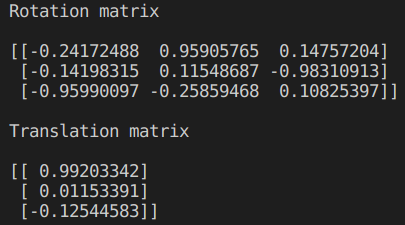
\includegraphics[width=\columnwidth]{/RT.png}
			\caption{Rotation and Translation of curule image}
			\label{fig:rt}
		\end{figure}
		
		
		\section{Rectification}
		
		I computed the epipolar lines and plotted it for both the images. 
		
		
		\begin{figure}[H]
			\centering
			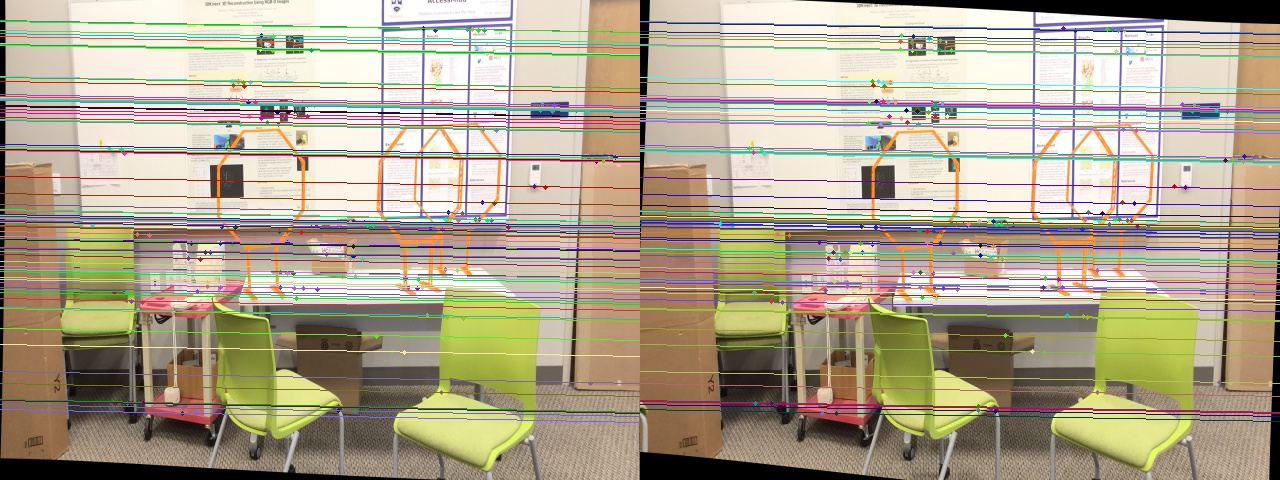
\includegraphics[width=\columnwidth]{/octagon_epipolar_lines.jpg}
			\caption{Depth image of octagon}
		\end{figure}
		
		Using homography matrix obtained for each images, I used warpPerspective to change the scene to straight view, shown in Figure \ref{fig:octagon_straight}.
		
		\begin{figure}[H]
			\centering
			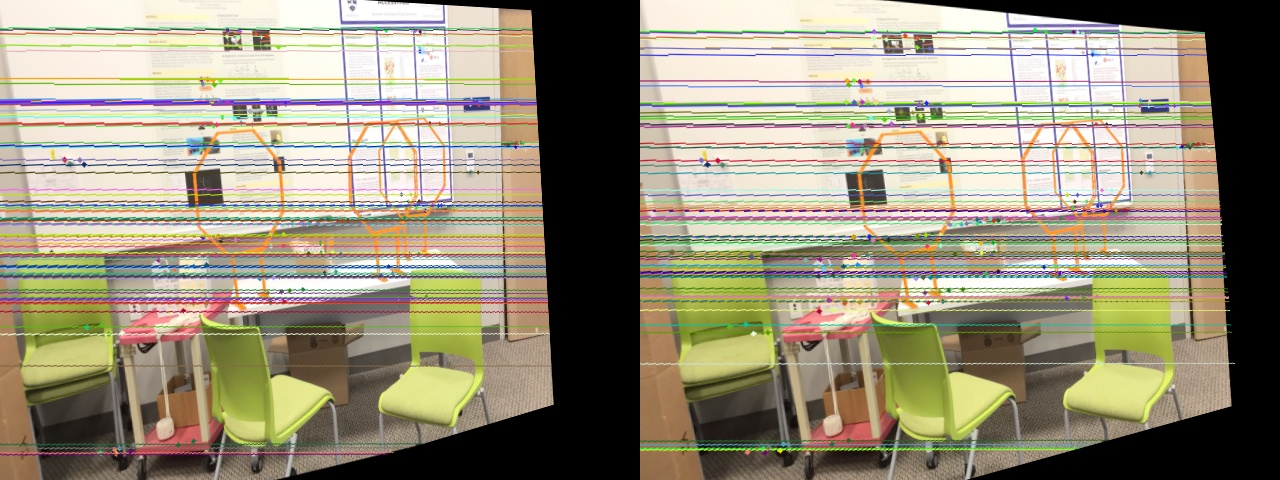
\includegraphics[width=\columnwidth]{/octogon_rectified.jpg}
			\caption{Depth image of octagon}
			\label{fig:octagon_straight}
		\end{figure}
	
	
		
		\section{Correspondence}	
		Before I calculate the disparity, I noticed that I had to align both images, I had to translate one of them. However, the scale was also off as well, the x axis of the image was squished. Hence, I did another feature matching both the rectified images using homography as shown in Figure \ref{fig:octagon_aligned}. 
		
		\begin{figure}[H]
			\centering
			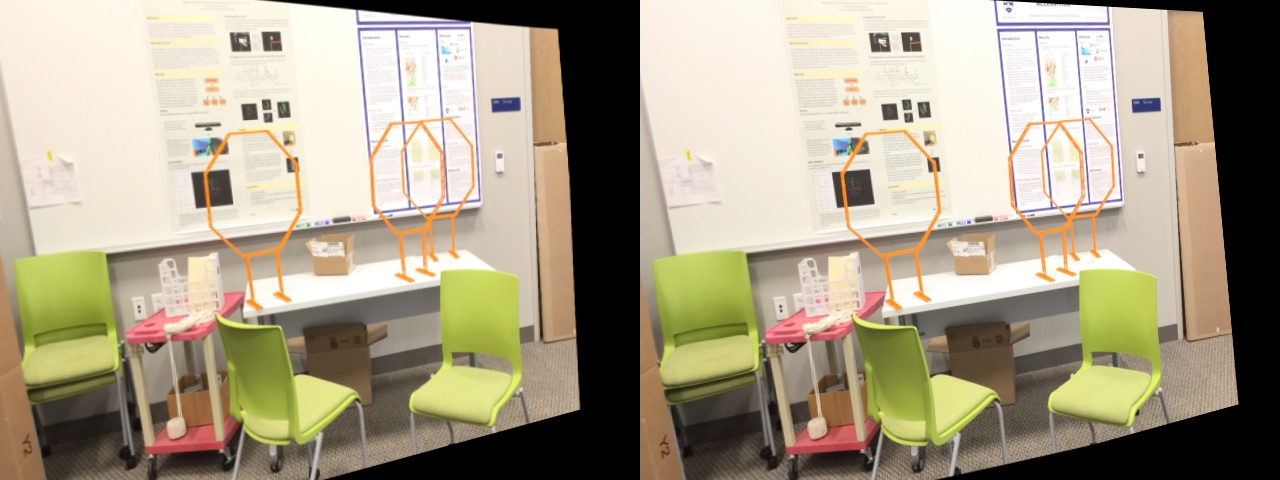
\includegraphics[width=\columnwidth]{/octagon_rectified_aligned.jpg}
			\caption{Aligned image of octagon}
			\label{fig:octagon_aligned}
		\end{figure}
		
		Then, I used window matching method to find the least difference to locate a pixel in its righ-hand side image counterpart. The window matching formula I used was $p = min|w_{l}-w_{r}|)$, where $p$ is the $(x,y)$ coordinates of the best pixel match. I tested various window sizes ranging from 5 to 20 pixels. Using a larger window size gave a reliable but dilated depth map, I used window size of 20 for curule image as shown in Figure \ref{fig:curule_depth_gray}. Using smaller window size give a finer resolution as shown in Figure \ref{fig:octa_depth_color}. For octagon, I used a smaller window size of 5, because of the thin edges of the octagon, it can be better located.
		
		
		\begin{figure}[H]
			\centering
			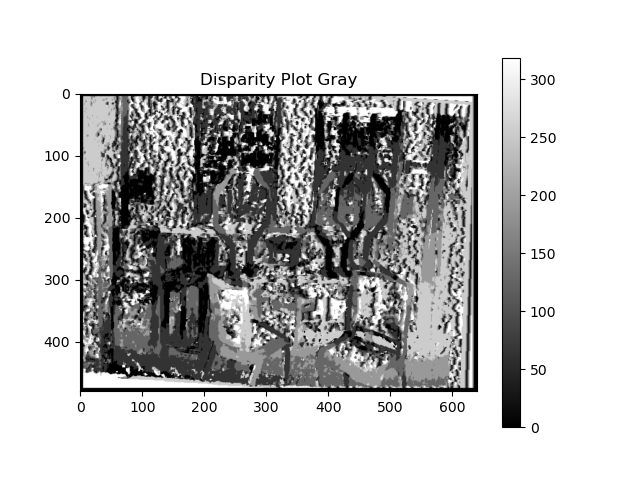
\includegraphics[width=\columnwidth]{/octagon_disparity_image_gray.png}
			\caption{Disparity gray image of octagon}
			\label{fig:octagon_disparity_gray}
		\end{figure}
		
		\begin{figure}[H]
			\centering
			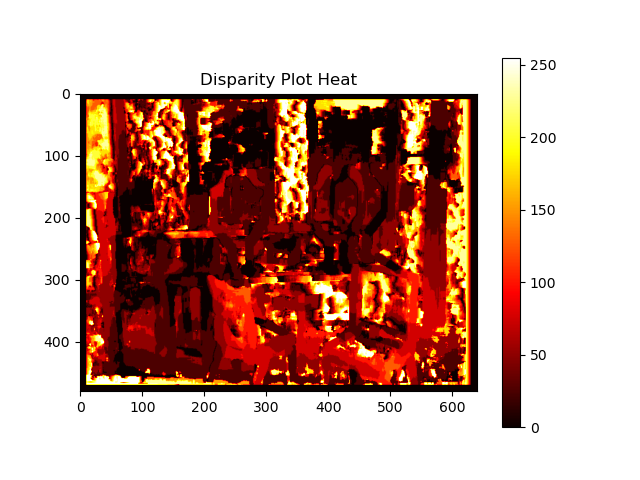
\includegraphics[width=\columnwidth]{/octagon_disparity_image_heat.png}
			\caption{Disparity color image of octagon}
			\label{fig:octagon_disparity_color}
		\end{figure}
		
		
		\section{Compute Depth Image}
		I computed the depth using the following equation, using baseline $B$, focal point $f_{x}$ and disparity $d$ :
		\[depth = \frac{Bf_{x}}{d}\]
		
		 From Figure \ref{fig:octa_depth_color}, we can see that the chair is in the front(very light orange), followed by the lone octagon(darker shade of orange), followed by 2 other octagons(dark purple). We can also see that the left most chair is further away than the middle chair, and this region of the image is different from the disparity image in Figure \ref{fig:octagon_disparity_color}.
	 
		\begin{figure}[H]
		\centering
		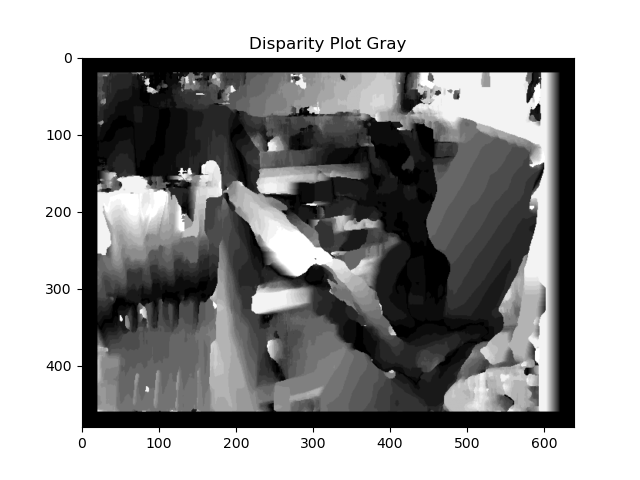
\includegraphics[width=\columnwidth]{/disparity_image_gray_curule.png}
		\caption{Depth image of curule}
		\label{fig:curule_depth_gray}
		\end{figure}



		\begin{figure}[H]
			\centering
			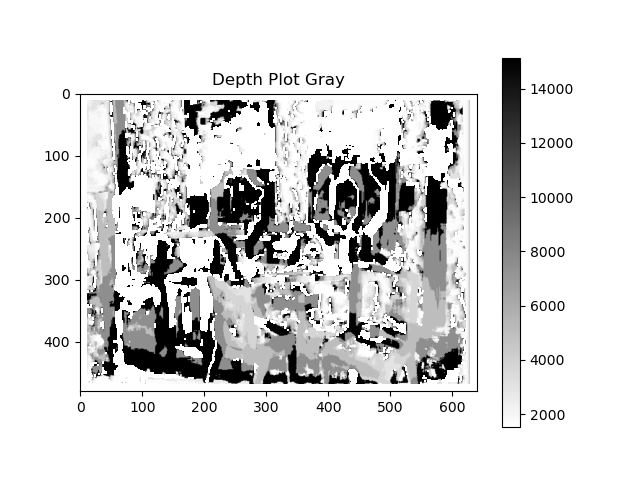
\includegraphics[width=\columnwidth]{/octagon_depth_gray.png}
			\caption{Depth gray image of octagon}
			\label{fig:octa_depth_gray}
		\end{figure}

		\begin{figure}[H]
		\centering
		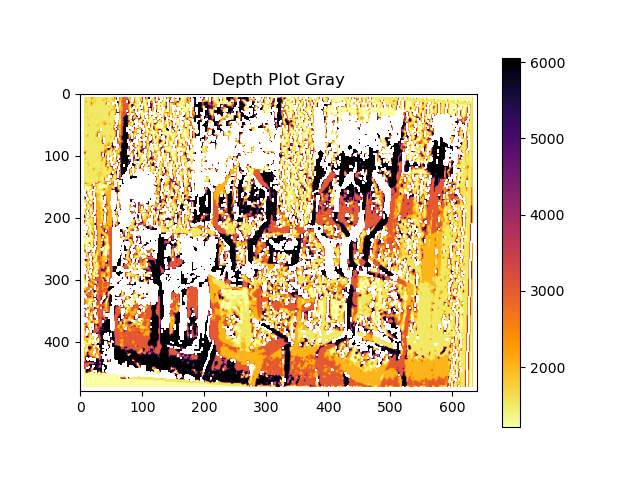
\includegraphics[width=\columnwidth]{/octagon_depth_color.png}
		\caption{Depth color image of octagon}
		\label{fig:octa_depth_color}
		\end{figure}
	
	
		\begin{figure}[H]
			\centering
			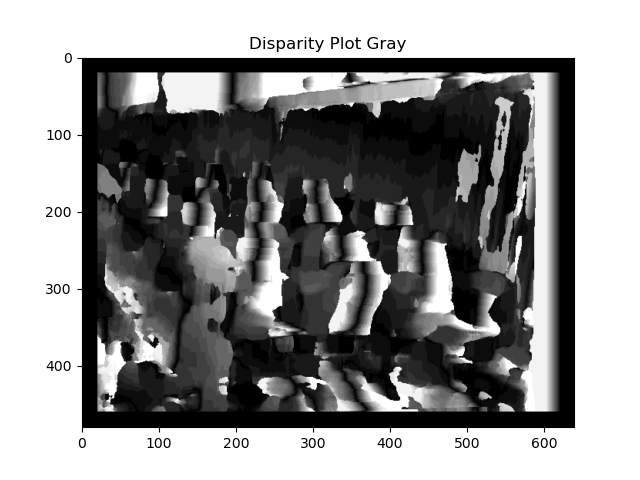
\includegraphics[width=\columnwidth]{/disparity_image_gray_pendulum.png}
			\caption{Depth image of pendulum}
			\label{fig:pendulum}
		\end{figure}
	
		\section{Conclusion}
		I calculated the dense depth map of images taken from different poses. This project taught me topics about Fundamental and Essential Matrix.
		
		
	\end{multicols}
	
	
	
\end{document}
